\documentclass[11pt, oneside]{article} 
\usepackage{geometry}
\geometry{letterpaper} 
\usepackage{graphicx}
	
\usepackage{amssymb}
\usepackage{amsmath}
\usepackage{parskip}
\usepackage{color}
\usepackage{hyperref}

\graphicspath{{/Users/telliott_admin/Tex/png/}}
% \begin{center} 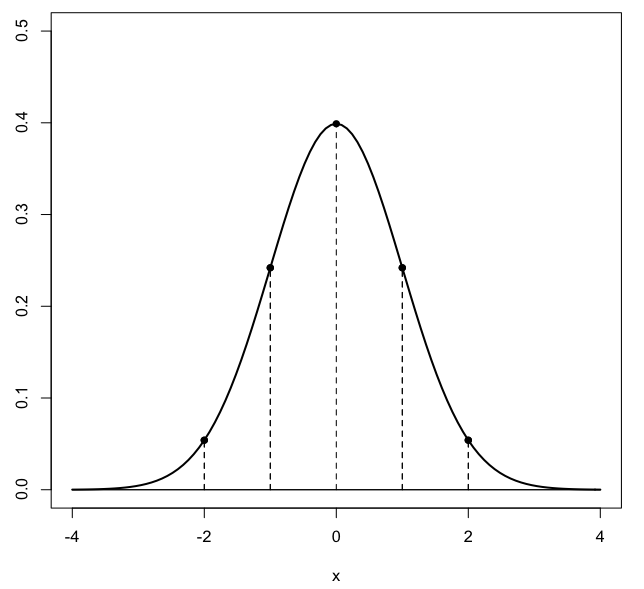
\includegraphics [scale=0.4] {gauss3.png} \end{center}

\title{Imaginary roots}
\date{}

\begin{document}
\maketitle
\Large
One can tell at least roughly where the roots of a polynomial are from the graph of the equation --- they are simply the points where the graph crosses the $x$-axis.

We can find them algebraically.

\subsection*{quadratic}
The general form of the quadratic is
\[ y = f(x) = ax^2 + bx + c \]
The roots are those values of $x$ that give $f(x) = 0$
\[ 0 = ax^2 + bx + c \]
\[ - \frac{c}{a} = x^2 + \frac{b}{a}x \]

\emph{The} quadratic formula (which gives the roots) is obtained by completing the square.

We guess the correct amount to add to both sides
\[ (\frac{b}{2a})^2 - \frac{c}{a} = x^2 + \frac{b}{a}x + (\frac{b}{2a})^2 \]

This helps because the right-hand side is now a perfect square
\[ (\frac{b}{2a})^2 - \frac{c}{a} = (x + \frac{b}{2a})^2 \]

Multiply the $c/a$ term on top and bottom by $4a$:
\[ (\frac{b}{2a})^2 - \frac{4ac}{(2a)^2}  = (x + \frac{b}{2a})^2 \]
Rearrange
\[ (x + \frac{b}{2a})^2 = (\frac{b}{2a})^2 - \frac{4ac}{(2a)^2}  \]
Put the right-hand side over a common denominator
\[ (x + \frac{b}{2a})^2 = \frac{b^2 - 4ac}{(2a)^2} \]
Take the square root
\[ x + \frac{b}{2a} = \pm \frac{\sqrt{b^2 - 4ac}}{2a}  \]
\[ x = \frac{-b \pm \sqrt{b^2 - 4ac}}{2a} \]

The first term of this looks familiar.  Going back to
\[ y = f(x) = ax^2 + bx + c \]
Take the derivative and set it equal to zero
\[ y' = 0 = 2ax + b \]
\[ x = \frac{-b}{2a} \]
This is the value of $x$ at the minimum (or maximum) value for the graph of $f(x)$.

Plugging that into the standard equation:
\[ y = a(\frac{-b}{2a})^2 + b(\frac{-b}{2a}) + c \]
\[ = \frac{b^2/2 - b^2}{2a} + c = \frac{- b^2}{4a} + c \]

\subsection*{discriminant}
The quantity under the square root is called the discriminant
\[ D = b^2 - 4ac \]
If $D > 0$, there are two roots, both real.

For example, a quadratic equation with $a > 0$ has a graph that opens up.  It has two real roots if the vertex is below the $x$-axis.  The condition for this is $D > 0$.

If the graph just touches the $x$-axis, there is a repeated root.  This happens when $D = 0$, and we can see from the quadratic formula above that the root is also the minimum.

There are no real roots if $D < 0$, because of the negative square root.  Graphically, this happens when the curve is shifted up (by making $c$ larger) so that the value of the function at the vertex is positive.

\subsection*{imaginary roots}

Nahin tells us that we can determine something about complex roots from the graph as well.  I'd never heard of that before.

Consider the plot of a general quadratic with $a > 0$ and negative discriminant ($b^2 - 4ac < 0$).  

\begin{center} 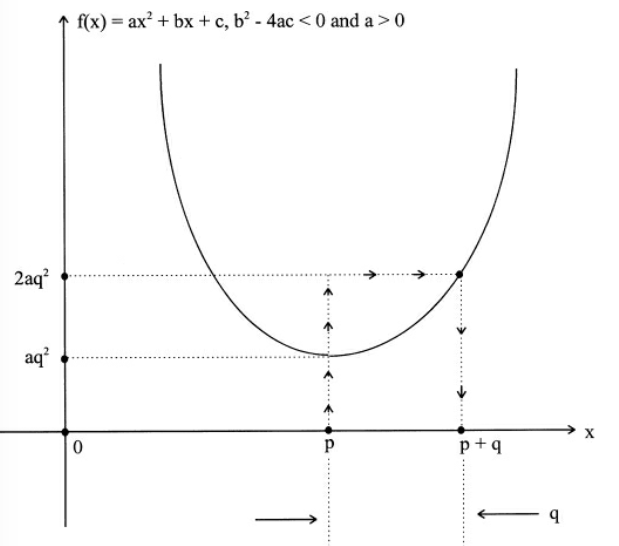
\includegraphics [scale=0.4] {roots1.png} \end{center}
The roots are complex conjugates of the form $p \pm iq$, and can be obtained from the quadratic equation.

Write $f(x)$ in \emph{factored} form:
\[ f(x) = a \ [ x - (p + iq) \ ] \ [ \ x - (p - iq) \ ] \]
\[ = a \ [ \ (x - p - iq)(x - p + iq) \ ]  \]
Multiplying out

\[ = a \ [ \ x^2 - px - iqx - px + p^2 + ipq + iqx - ipq + q^2 \ ] \]
\[ = a \ [ \ x^2 - 2px + p^2 + q^2 \ ] \]
\[ = a \ [ \ (x-p)^2 + q^2 \ ] \]

This expression is entirely real.

The value of $f(x)$ is clearly a minimum when $x = p$.  

$p$ is also the real part of the complex roots.  At the minimum $x = p$ and the $y$-value is equal to $aq^2$.

When $x = p + q$, $f(x) = 2aq^2$.

Geometrically, one can think about measuring the displacement from the $x$-axis at the minimum.

Then, find the point where the displacement is twice that, and find the corresponding change in $x$ from the vertex.

All it takes is a ruler and pencil.

\subsection*{cubic}

Suppose we have a cubic with only one real root, $x = k$, and a pair of conjugate roots $x = p \pm iq$.  The factored form of the cubic is

\[ f(x) = (x - k)(x - p + iq)(x - p - iq) \]
We already did this exact multiplication, above
\[ = (x - k)(x^2 - 2xp + p^2 + q^2) \]

\begin{center} 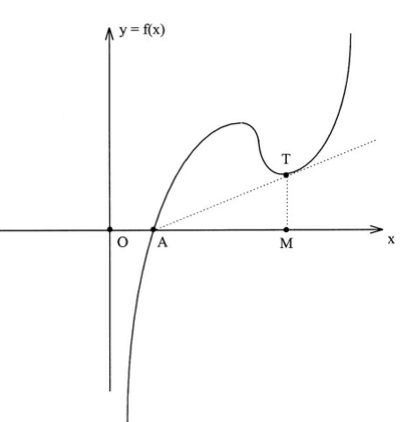
\includegraphics [scale=0.4] {roots2.png} \end{center}
The equation of a line going through the real root at $(k,0)$ is 
\[ \frac{\Delta y}{\Delta x} = \frac{y}{x - k} = \lambda \]
where $\lambda$ is the slope.  So
\[ y = \lambda (x - k) \]

We are interested in one particular line, one with slope such that it just touches the curve to be a tangent, at $T$ above.  

At the point of tangency we have the displacement of $x$ from the root as $x = \hat{x}$ and write
\[ \lambda (\hat{x} - k) = (\hat{x} - k)(\hat{x}^2 - 2p\hat{x} + p^2 + q^2) \]

Since $(\hat{x} - k) \ne 0$, we can divide to give:
\[ \lambda = \hat{x}^2 - 2p\hat{x} + p^2 + q^2 \]
\[ \hat{x}^2 - 2p\hat{x} + p^2 + q^2 - \lambda = 0 \]

This is a quadratic in $\hat{x}$.  Moreover, since the line just touches the curve, we are at the point where the discriminant is equal to zero.  That is

\[ 4p^2 - 4(p^2 + q^2 - \lambda) = 0 \]
That is
\[ - 4(q^2 - \lambda) = 0 \]
\[ \lambda = q^2 \]

The tangent line has slope $\lambda = q^2$.

The value of $\hat{x}$ can then be computed from
\[ \hat{x}^2 - 2p\hat{x} + p^2 + q^2 - \lambda = 0 \]
Since $\lambda = q^2$:
\[ \hat{x}^2 - 2p\hat{x} + p^2  = 0 \]
\[ (\hat{x} - p)^2 = 0 \]
\[ \hat{x} = p \]

Geometrically, use a straight-edge to construct the line and find the tangent point.  $q$ is the square root of the slope of this line.  This is the quantity $TM/AM$.

The $x$ displacement of $T$ from the real root is $p$.  This is the quantity $AM$.

\begin{center} 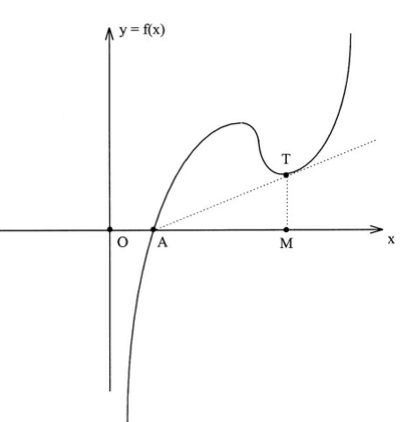
\includegraphics [scale=0.4] {roots2.png} \end{center}

\end{document}